\documentclass[
    11pt,
    a4paper,
    egregdoesnotlikesansseriftitles,
    toc=chapterentrywithdots,
    twoside,openright,
    titlepage,
    parskip=half,
    headings=normal,  % reduces heading size
    listof=totoc,
    bibliography=totoc,
    index=totoc,
    captions=tableheading,  % caption below table
    chapterprefix,
    listof=flat,
    final
]{scrbook}


% details about your thesis
\newcommand{\titel}{Enablement of Kubernetes Based Open-Source Projects on IBM Z}
\newcommand{\artderarbeit}{Bachelor Thesis}  % {Bachelorarbeit,Masterarbeit}
\newcommand{\autor}{Sarah Julia Kriesch}
\newcommand{\studiengang}{Informatik}  % {Informatik,Wirtschaftsinformatik,Medieninformatik}
\newcommand{\matrikelnr}{303\,6764}
\newcommand{\erstgutachter}{Prof.\,Dr.~Ralf\,Ulrich Kern}
\newcommand{\zweitgutachter}{Prof.\,Dr.~Tobias Bocklet}
\newcommand{\betreuer}{~Alice Frosi}
\newcommand{\logo}{figures/TH-Nuernberg-RGB.png}
\newcommand{\keywords}{Hardware Emulation, Apache Cassandra, Kubernetes, Open Source, Linux on Z, IBM Z, Mainframes}
 

% custom head and foot
\usepackage[automark]{scrlayer-scrpage}
\pagestyle{scrheadings}
\ihead{\headmark}
\chead{}
\ohead{\pagemark}
\renewcommand*\chaptermarkformat{\chapappifchapterprefix{\ }% 
  \thechapter.\enskip}

\RedeclareSectionCommand[tocindent=0pt]{section}
\RedeclareSectionCommand[tocindent=0pt]{subsection}
%\RedeclareSectionCommand[tocnumwidth=70pt]{chapter}

\usepackage{scrhack}

% other packages
\usepackage[utf8]{inputenc}
\usepackage[T1]{fontenc}
\usepackage{lmodern,relsize,textcomp,csquotes}
\usepackage{amsmath,amsfonts}
\usepackage[ngerman,english]{babel}  % flip for German thesis
\usepackage[final]{graphicx}
\usepackage{setspace,geometry,xcolor}
\usepackage{makeidx}
\usepackage{paralist,ifthen,todonotes}
\usepackage{url}
\usepackage{pdfpages}
\usepackage{microtype}


% table setup
\usepackage{longtable}
\usepackage{array}
\usepackage{ragged2e}
\usepackage{lscape}

% pdf hyperref
\usepackage[
    bookmarks=true,
    bookmarksopen=true,
    bookmarksnumbered=true,
    bookmarksopenlevel=1,
    pdftitle={\titel},
    pdfauthor={\autor},
    pdfcreator={\autor},
    pdfsubject={\titel},
    pdfkeywords={\keywords},
    pdfpagelabels=true,
    colorlinks=true,
    linkcolor=red,
    urlcolor=magenta,
    anchorcolor=black,
    citecolor=cyan,
    filecolor=magenta,
    menucolor=red,
    plainpages=false,
    hypertexnames=true,
    linktocpage=true,
]{hyperref}


% configure your listings style
\usepackage{listings}
\lstset{
	tabsize=3,
	extendedchars=true,
	frame=single,
	showstringspaces=true,
	numbers=left,
	numberstyle=\small,
	breakautoindent=true
}

% page setup
% \setlength{\topskip}{\ht\strutbox}
\geometry{paper=a4paper,left=2.5cm,top=3.0cm,bindingoffset=.8cm}
\onehalfspacing
\frenchspacing
\clubpenalty = 10000
\widowpenalty = 10000 
\displaywidowpenalty = 10000

% some commands
\newcommand{\ua}{\mbox{u.\,a.\ }}
\newcommand{\zB}{\mbox{z.\,B.\ }}
\newcommand{\dahe}{\mbox{d.\,h.,\ }}
\newcommand{\bzw}{\mbox{bzw.\ }}
\newcommand{\bzgl}{\mbox{bzgl.\ }}
\newcommand{\eg}{\mbox{e.\,g.\ }}
\newcommand{\ie}{\mbox{i.\,e.\ }}
\newcommand{\wrt}{\mbox{w.\,r.\,t.\ }}
\newcommand{\etal}{\mbox{\emph{et.\,al.\ }}}


% TODO remove if not needed...
\usepackage{blindtext}


\begin{document}

\setcounter{secnumdepth}{3}  % numerate subsections
\setcounter{tocdepth}{2}  % ...but don't include them in toc

\frontmatter
\thispagestyle{empty}
\pdfbookmark[1]{Cover}{cov}
\begin{titlepage}

\begin{center}


\includegraphics[width=\linewidth]{figures/TH-Nuernberg-RGB.png}\\[1cm]
\LARGE{Fakultät Informatik}\\[2cm]

\huge
\textbf{\titel}\\[1cm]
%
\Large
\artderarbeit~im Studiengang \studiengang\\[1cm]
%
\large
vorgelegt von

\Large
\autor\\[0.5cm]
\small
Matrikelnummer \matrikelnr\\[2cm]

\vspace*{\fill}

\large
\begin{tabular}{p{3cm}p{8cm}}\\
Erstgutachter:  & \quad \erstgutachter\\[1.2ex]
Zweitgutachter: & \quad \zweitgutachter\\[1.2ex]
Betreuer: & \quad \betreuer\\
Unternehmen: & \quad \unternehmen

\includegraphics[width=\linewidth]{figures/ibm-logo.pdf}
\end{tabular}
\end{center}

\begin{center}
\copyright\,\the\year
\end{center}

\vspace{-0.5cm}
\singlespacing
\small
\noindent Dieses Werk einschließlich seiner Teile ist \textbf{urheberrechtlich geschützt}.
Jede Verwertung außerhalb der engen Grenzen des Urheberrechtgesetzes ist ohne Zustimmung des Autors unzulässig und strafbar.
Das gilt insbesondere für Vervielfältigungen, Übersetzungen, Mikroverfilmungen sowie die Einspeicherung und Verarbeitung in elektronischen Systemen.

\end{titlepage}
\cleardoublepage

% download the following form and complete it (hit save in your editor)
% https://intern.ohmportal.de/fileadmin/Gelenkte_Doks/Abt/SZS/SB/SB_0050_FO_Pruefungsrechtliche_Erklaerung_und_Erklaerung_zur_Veroeffentlichung_der_Abschlussarbeit_public.pdf
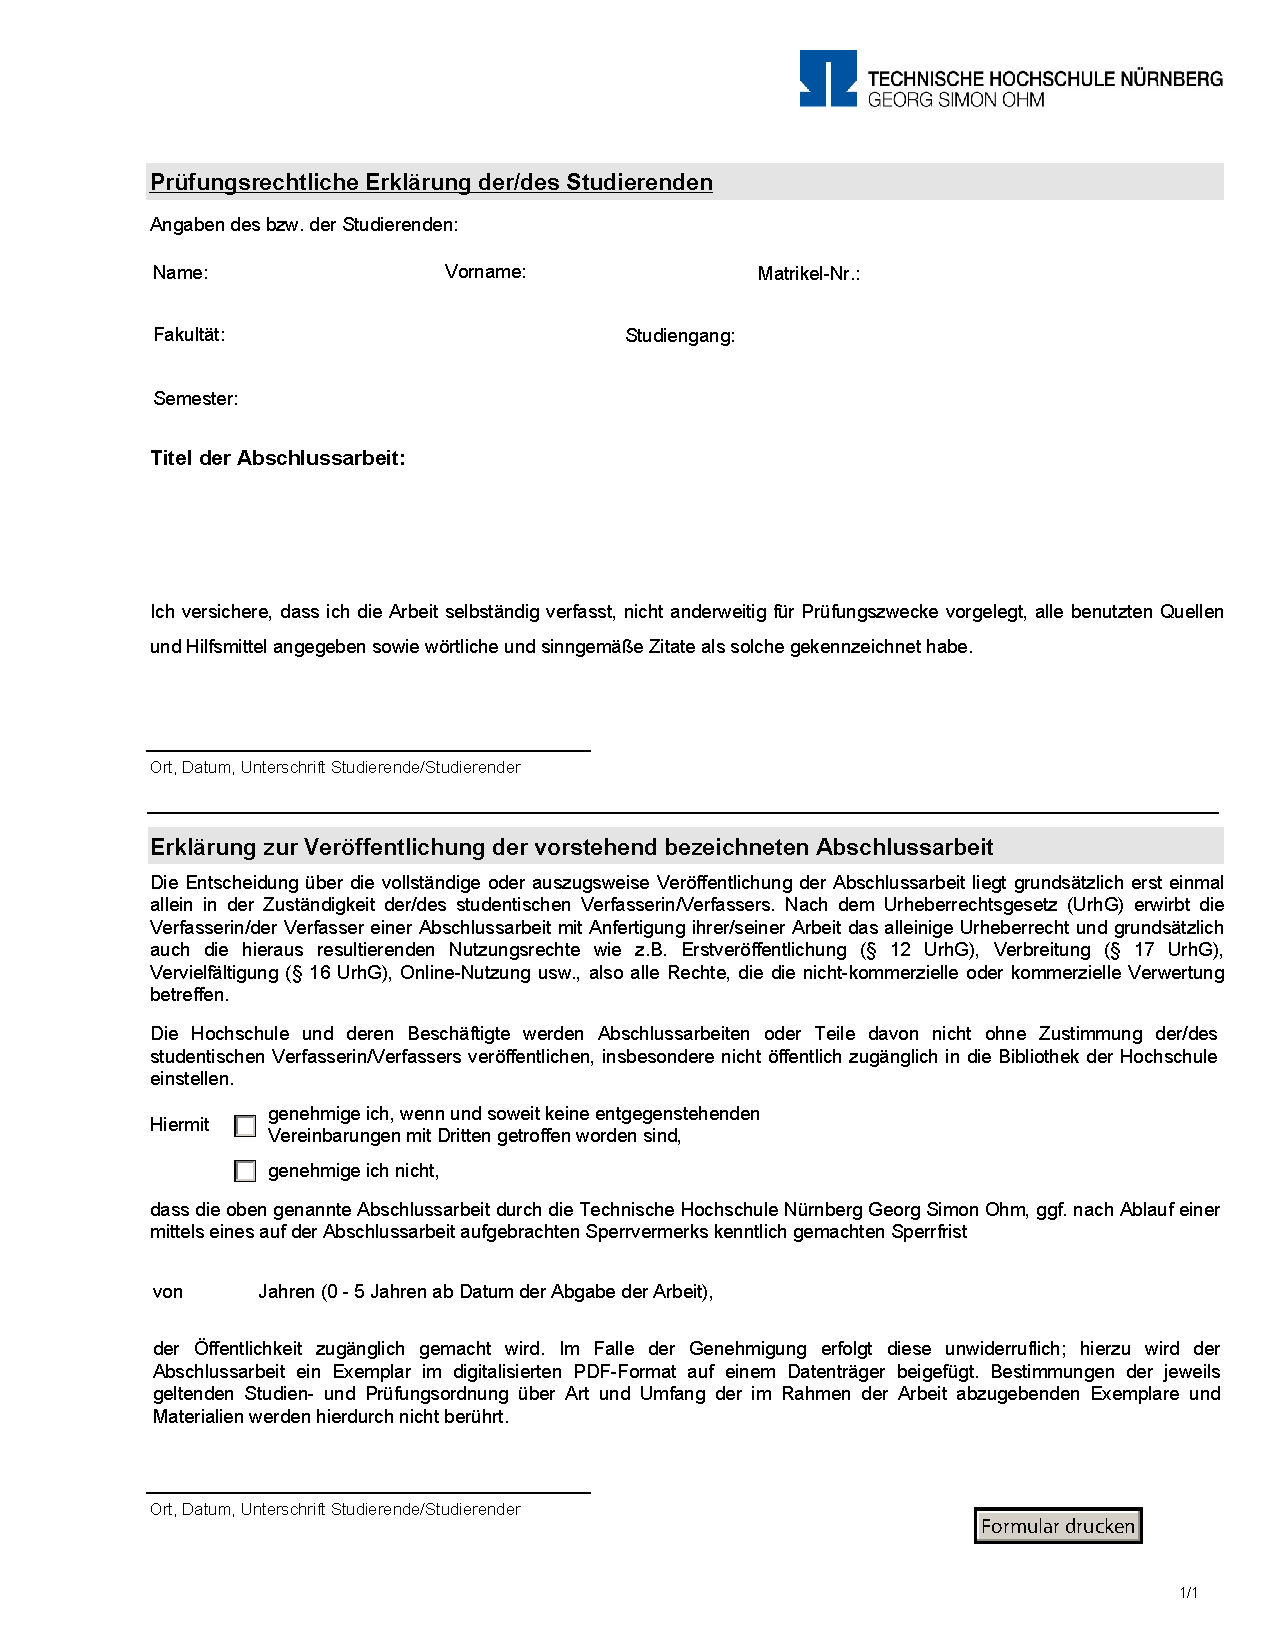
\includepdf{SB_0050_FO_Pruefungsrechtliche_Erklaerung_und_Erklaerung_zur_Veroeffentlichung_der_Abschlussarbeit_public.pdf}\cleardoublepage

\thispagestyle{empty}
\section*{Kurzdarstellung}
\label{sec:kurzdarstellung}
%Kurze Zusammenfassung der Arbeit, höchstens halbe Seite.
Open-Source-Projekte entwickeln Software, bei der der Quellcode frei verfügbar ist. Diese Communitys lassen automatisierte Tests gegen jede Code-Änderung laufen, um die bester Software-Qualität zu garantieren. 
Diese Tests sollen auf unterschiedlichen Architekturen laufen können. Es ist schwierig, Software für grundlegende Hardware ohne Zugriff darauf zu testen. Deshalb muss die in IBM Z verwendete s390x-Architektur für ausgewählte Open-Source-Projekte emuliert (nachgeahmt) und in die entsprechende CI/CD-Pipeline eingefügt werden. 
Das sollte mit schnellen Deployment-Methoden im Emulator QEMU durchgeführt werden. 
Kubernetes wird als containerisiertes Beispiel-Projekt als Grundlage für dafür eingeführte Anwendungen verwendet. Ein weiteres Open-Source-Projekt, Apache Cassandra, wird verwendet um Tests auf der Anwendungsschicht im Kubernetes-Stack zu repräsentieren. \\
Zusätzlich müssen die minimalen Systemanforderungen für die Einrichtung innerhalb der CI/CD-Infrastruktur beider Projekte wegen der Minimierung an Festplattenplatz, Memory und CPU-Verbrauch analysiert werden. \\
Zum Abschluss wird die automatische Emulation beider Projekte in die Test-Infrastruktur integriert, so dass diese Projekte für die s390x-Architektur von IBM Z Mainframes aktiviert sind. Allgemein soll diese Methode für weitere Open-Source-Projekte in der Zukunft wiederverwendet werden können.



\section*{Abstract}
\label{sec:abstract}

Open-source projects are developing software with freely available source code. These communities are running automated tests against every code change in order to guarantee the best software quality. 
These tests should be able to run on different architectures. It is difficult to test software for essential hardware without access. Therefore, the \gls{s390x} architecture used in IBM Z has to be emulated on x86 for chosen open-source projects and included in their \gls{CI/CD} pipeline. 
That should be executed with fast deployment methods in the \gls{emulator} QEMU. 
Kubernetes is used as a \gls{containerized} example project as the foundation for instituting applications. Another open-source project, Apache Cassandra, is applied to represent tests on the \gls{application layer} in the Kubernetes stack. \\
Additionally, minimal system requirements have to be analyzed for the setup inside of the CI/CD infrastructure of both projects concerning the minimization of disk space, memory and CPU usage for deployments. \\
Finally, the automated emulation of both projects will be integrated into the test infrastructure, so that these projects are enabled for the s390x architecture of \gls{IBM Z systems}. Overall, this method should be reusable for further open-source projects in the future.


\cleardoublepage

\tableofcontents

\mainmatter
\chapter{Introduction}\label{ch:intro}


\blindtext

\section{Container Orchestration}

\blindtext

\subsection{Kubernetes}

Kubernetes\footnote{\url{https://kubernetes.io/}} is an open-source project for container orchestration. That is well known as K8s, too. This project was started by Google. A Kubernetes cluster has at least one Master node and one Worker node for high availability. This container platform portable for private und public clouds. Kubernetes is available as a managed platform by different cloud providers as same as different Kubernetes distributions exist to download or installations from scratch are possible. It is configurable with different container runtimes, as Docker\footnote{\url{https://www.docker.com/}}, Podman\footnote{\url{https://podman.io/}} or CRI-O\footnote{\url{https://cri-o.io/}} as examples. The Container Runtime Interface (CRI) is necessary for managing container images, the life cycle of container pods, networking and help functions\cite[~p.16]{Scholl2019}. 
\blindtext

\section{Mainframe Computers}

Mainframe computers are large computers. Some of them are part of the Z series\footnote{\url{https://www.ibm.com/it-infrastructure/z/hardware/}} by IBM. They are not only used as internet servers or for banking systems. They can handle large numbers of transactions in one second for e-commerce\cite[~p.56]{Tanenbaum2014}. Such Z systems do not use the well known x86 architecture. They are built with s390x. This architecture has been developed by IBM. It has been introduced in late 2000 and supported by the Linux Kernel since late 1999\cite[~p.15]{Block2019}. The traditional operating system for mainframes has been z\/OS. Linux is used as a base operating system for this Bachelor Thesis.


\blindtext

\section{Hardware Emulation}

Not everybody has access to expensive hardware or hardware with  specific architecture. Software should be able to run on most important hardware architectures. The solution for Software Developers is hardware emulation. You can test based on hypervisors with the hardware emulation whether the software is running correctly.
\blindtext

\section{Open Source Projects}
\blindtext

\subsection{And an even more important subsection}
\blindtext

\chapter{Data}\label{ch:data}

\Blindtext

\chapter{Method}\label{ch:method}

In this chapter, we're actually using some code!

\begin{lstlisting}[language=Python,caption={This is an example of inline listing},captionpos=b]
x = 1
if x == 1:
    # indented four spaces
    print("x is 1.")

\end{lstlisting}

You can also include listings from a file directly:

\lstinputlisting[language=Python,caption={This is an example of included listing},captionpos=b]{listings/example.py}

\chapter{Experiments}\label{ch:experiments}

\Blindtext

\chapter{Outlook}\label{ch:outlook}

\Blindtext

\chapter{Summary}\label{ch:summary}

\Blindtext


% remove if not needed
\appendix
\chapter{Supplemental Information}\label{app:supplemental-information}

\section{Circle CI configuration for Apache Cassandra}\label{CircleCI}
\begin{boxedverbatim}
jobs:
  build-docker-image:
    working_directory: ~/s390x
    docker:
      - image: Dockerfile
    steps:
      - attach_workspace:
          at: .
      
      - run: 
            name: Build for s390x
            command: docker build buildx --platform=linux/s390x --squash \
                    -t cassandra:s390x .
      - docker/check:
         registry: $DOCKER_REGISTRY 
  prepare-kernel:
    steps:
        - run:
              name: Fetching the Linux kernel
              command: |
                      mkdir ~/s390x/kernel-bionic; debootstrap --include=linux-generic \
                      --arch=s390x --variant=minbase bionic kernel-bionic \
                      http://ports.ubuntu.com
        - store_artifacts:
              path: ~/s390x/kernel-bionic/boot/vmlinuz-4.15.0-20-generic
        - persist_to_workspace:
                  root: .
                  paths:
                      - .
        
\end{boxedverbatim}

\begin{boxedverbatim}
  prepare-filesystem:
    working_directory: ~/s390x
      steps:
        - attach_workspace:
                  at: .
        - run:
              name: Creating a ext4 filesystem with integration of the Cassandra image
              command: |
                      mkdir rootfs; qemu-img create -f raw cassandra-s390x.img \
                      $(docker images | grep 'cassandra:s390x' | \
                      awk '{print int($7+0.5)"G"}'); \
                      docker export $(docker create cassandra:s390x)| \
                      tar -C "rootfs"-xvf -;  mkfs.ext4 -F cassandra-s390x.img;\
                       mount -o loop cassandra-s390x.img /mnt/rootfs; \
                      cp -r rootfs/* /mnt/rootfs/.
        - store_artifacts:
              path: ~/s390x/cassandra-s390x.img
  test:
  working_directory: ~/s390x
    steps:
      - attach_workspace:
                  at: .
      - run:
             name: Run test with QEMU
             command: |
                     /usr/bin/qemu-system-s390x -kernel vmlinuz-4.15.0-20-generic \
                     -m 4G -M s390-ccw-virtio -nodefaults -device sclpconsole,\
                     chardev=console -parallel none -net none -chardev stdio,\
                     id=console,signal=off,mux=on -mon chardev=console \
                     -nographic -smp 3 -hda cassandra-s390x.img \
                     --append ’root=/dev/vda rw console=ttyS0 rdinit=/bin/bash’  
workflows:
    version: 1
    build-test:
      jobs:
        - prepare-kernel
        - build-docker-image
              requires: 
                  - prepare-kernel
        - prepare-filesystem
              requires: 
                  - build-docker-image
        - test
             requires:
                 - prepare-kernel
                 - prepare-filesystem
\end{boxedverbatim}

\backmatter
\listoffigures
\cleardoublepage

\listoftables
\cleardoublepage

\renewcommand{\lstlistlistingname}{List of Listings}  % change for German thesis
\lstlistoflistings
\cleardoublepage

\bibliographystyle{wmaainf}
\bibliography{refs}

\end{document}
